\chapter{Implementation}
\label{cha:implementation}

Section 3 describes global requirements and a frame for the authentication and authorization framework implementation. This section will now explained how the IdP of \emph{device cloud} has been implemented, in a so-called User Directory.

\section{The Model}
Before explaining how authentication is done or how the application is structured, the model should be defined. As explained in the previous section, the model of the \emph{device cloud} comprehends at least the different principals and the so-called consumer profile. The other components of the model, like the Request (a client sends a request to the User Directory by serialzing a Request object) or RequestResult are not required for the understanding of the framework and will therefore not be presented.

As shown in Fig. \ref{fig:principals}, all the entities of the \emph{device cloud} derive from a generic Entity abstract class, which contains global attributes like EntityOperator (already discussed in section \ref{03_authorizing}) or EntityType (i.e. Operator, Consumer, etc) and a generic ID. The principal and the consumer profile classes will then extend this generic abstract Entity class, specifying at the same time the class of the generic field ID.

A Consumer could for instance be defined as an Entity whose ID is a String (like an email), whereas an Operator as an entity whose ID is a UID (Unique Identifier, i.e. a Long type). Both would still extend the Entity class and offers the same functionalities.

\subsection{The principals}
A Principal is defined as an entity, which inherits from the interfaces PrincipalEntity, ConfigurableEntity and AttachmentEntity, as one can see Tab \ref{tab:02_entities}, and whose ID is a PrincipalIdentifier. The PrincipalIdentifier class is a wrapper around a String identifier, which allows for various types of identifiers (GUID, email, alias) and offers conversation and type verification capabilities (a Globally unique identifier GUID or a UID should be a Long, an email should respect a certain format, etc).

Since a principal can be authenticated, it encompasses a \textit{secret} attribute, like a password, and a certificate (SSL authentication is required from the design). Attachments can be added (one could attach the certificate of the principal for example, as a file) and a configuration (set of key value pairs) can be also defined.

This abstract class is then extended into the Consumer, Vendor, Operator, and Aggregator classes. They all define the appropriate EntityType, the attributes defined beforehand (A ProtocolURI for the Operators for example), and, if required, they implement the Location Tagged Entity Interface, with which the location of a principal can be retrieved.

\begin{figure}[!hpbt]
	\centering
	\caption{Principal model}
	\label{fig:principals}
	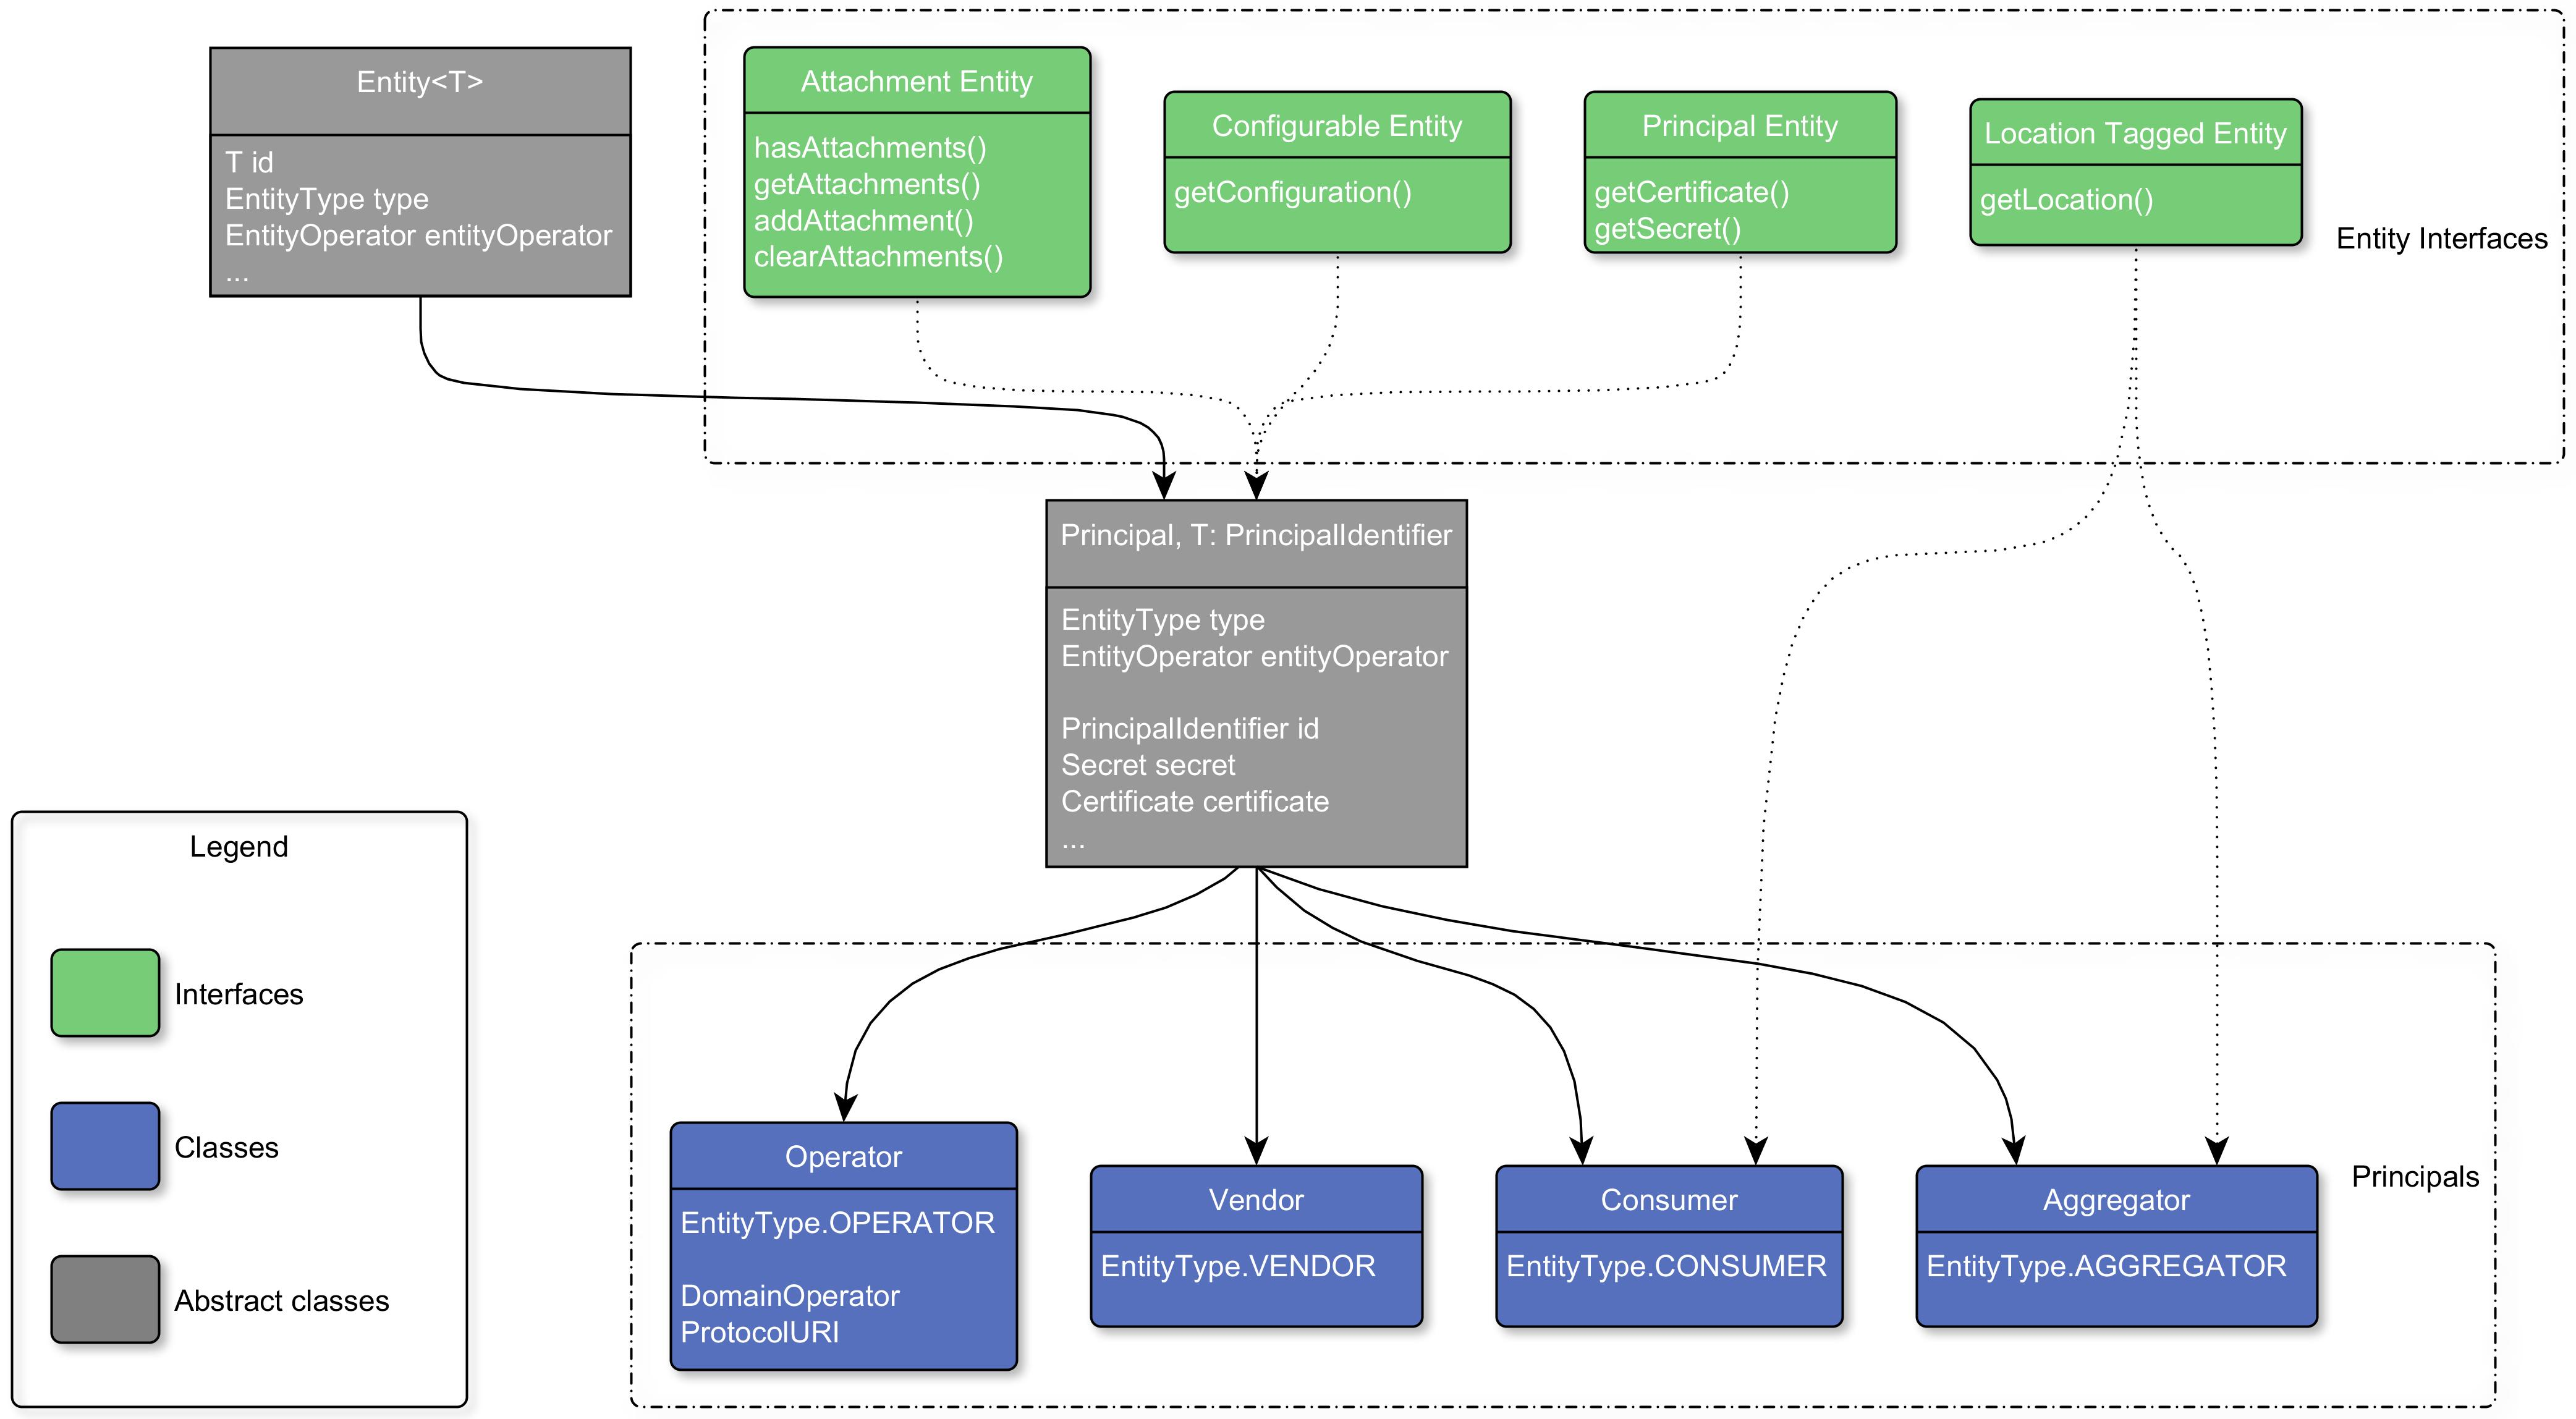
\includegraphics[width=1\textwidth]{images/principals}
\end{figure}

\subsection{The consumer profile}
The consumer profile implementation has been already partially described in the \citetitle{reference_thesis}:
the consumer profile defines a set of software modules and a set of paths between those to enable automatic deployment of a chain of modules. Operations like automatic data format conversion could for example be achieved easily, by adding a converter module between the raw data of the device and the output. 

Such paths of software modules logically always refers to a specific device category (blood pressure, glucose meter, etc). Therefore, the paths are grouped within entries. The consumer profile defines those entries, each bound to a specific device category and describing node paths. For a specific device category, an entry can be then best described as "a directed acyclic graph, which defines the processing of a data stream".

Since the same module can be used in several entries and/or paths, but is deployed only once, it is put within a Node object, which regroups a module and an ID. The nodes are defined in the consumer profile with an unique ID, and the different entry paths will then just refer to the corresponding IDs. It must be here also noted that it is not the role of the User Directory to store direct information about devices, like software modules. Instead, information is stored, that is sufficient to retrieve the module, like an identifier (ModuleIdentifier).

Ultimately, the Consumer Profile defines a list of entities who are allowed to read it, as stated in section \ref{03_consumer_profile_authorization}. Only those entities can get the profile in order to, for instance, decide whether a new detected device is of interest or to deploy automatically a chain of modules.

With the example of the diabetic glucose meter introduced in section 2 (see \hyperref[02_consumer_profile_example]{consumer profile example}), the consumer profile would then be depicted as in Fig. \ref{fig:consumer_profile_example}. The first entry specifies the data conversion from a proprietary format to a standard CSV format. An second entry is rendered, only for representation purposes.

\begin{figure}[!hpbt]
	\centering
	\caption{Consumer Profile Example}
	\label{fig:consumer_profile_example}
	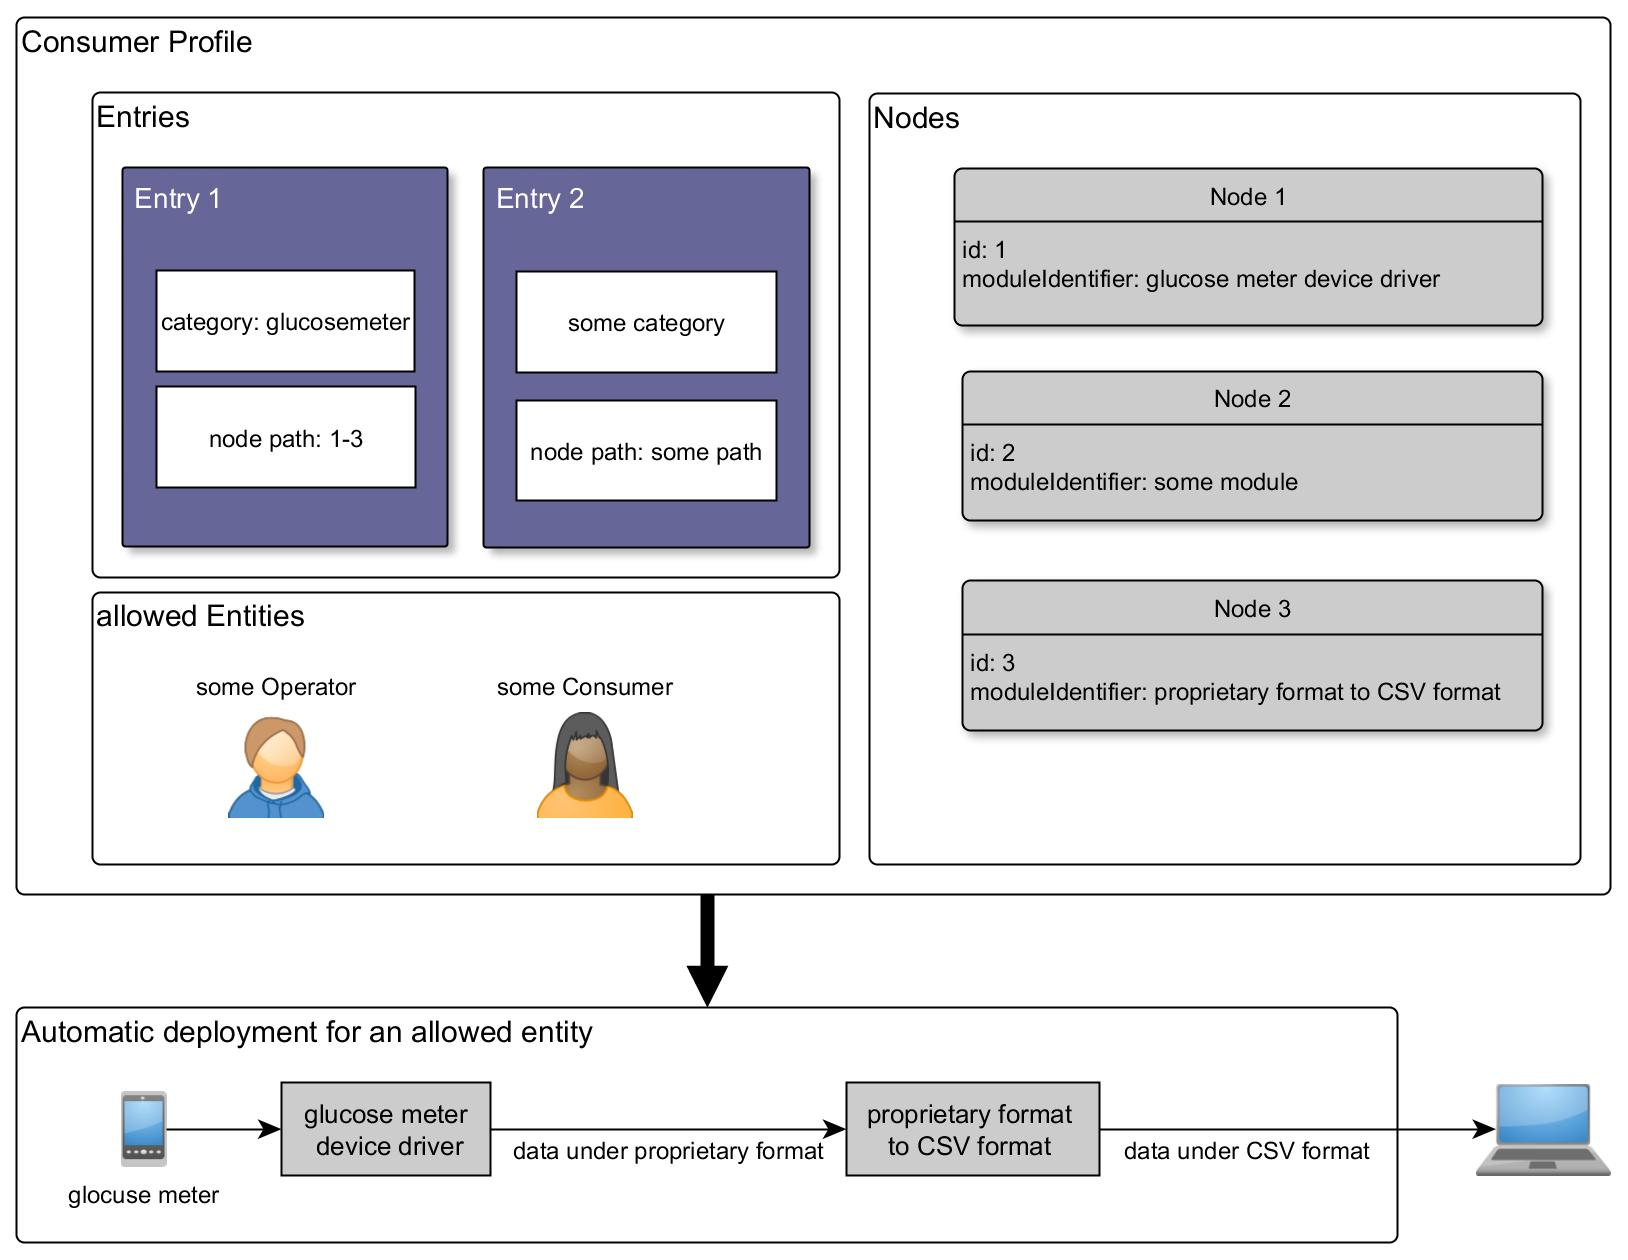
\includegraphics[width=1\textwidth]{images/consumer_profile_example}
\end{figure}

The consumer profile and the consumer profile entries, as they respectively express the consumer's preferences and a deployment scheme, requires to be highly configurable. Moreover, it is conceivable for both to be created, added, updated or removed directly from a user request (it is already the case for the consumer profile; one could consider this for the entries as well). For these reasons, both can be regarded as entities of the User Directory.

They inherit therefore from the interfaces ConfigurableEntity and AttachmentEntity defined in Tab. \ref{tab:entities_interface}, which means that files or sets of configuration key-value pair can be attached.

\section{Structure}
The User Directory has been structured to enhance re-usability and modularity, as shown in Fig. \ref{fig:code_struct}. Basically, a few interfaces and abstract classes have been defined that allow any security implementation to be plugged in as module:

\begin{description}
	\item[communication interface]: this is the communication layer of the application. It receives the requests of the clients, performs basic controls like checking authentication, parse the requests and call the good logic method with the appropriate arguments..\\
	\item[logic interface]: this interface performs the methods of the authentication and authorization framework defined  in the section \ref{sec:04_framework}. It calls the low-level services and coordinates them to handle any request from the clients.\\
	\item[authentication layer]: handles both type of authentication request, \textit{authenticate} and \textit{delegated authentication}. Implementations of those interfaces performs specific security framework operations, like OpenID Connect, Kerberos, etc..\\
	\item[persistence services] The authentication layer is placed on top of several data persistence services (at least two, one for the principal and one for the other entities) which allows for creating, removing, updating or simply getting entities from the persistence systems.
	\item[authorization layer]: since authorization is in the \emph{device cloud} performed only for modification or creation of persisted entities (see Tab. \ref{tab:access_control}), an authorization layer is added as support for the data persistence layer. It defines the right to create, read, remove or update a persisted entity for any principal. \\
	\item[session management]: session management is performed in parallel and provide the others component with an authentication context (who is authenticated, etc).
\end{description}


\begin{figure}[hpbt]
	\centering
	\caption{Structure of the project}
	\label{fig:code_struct}
	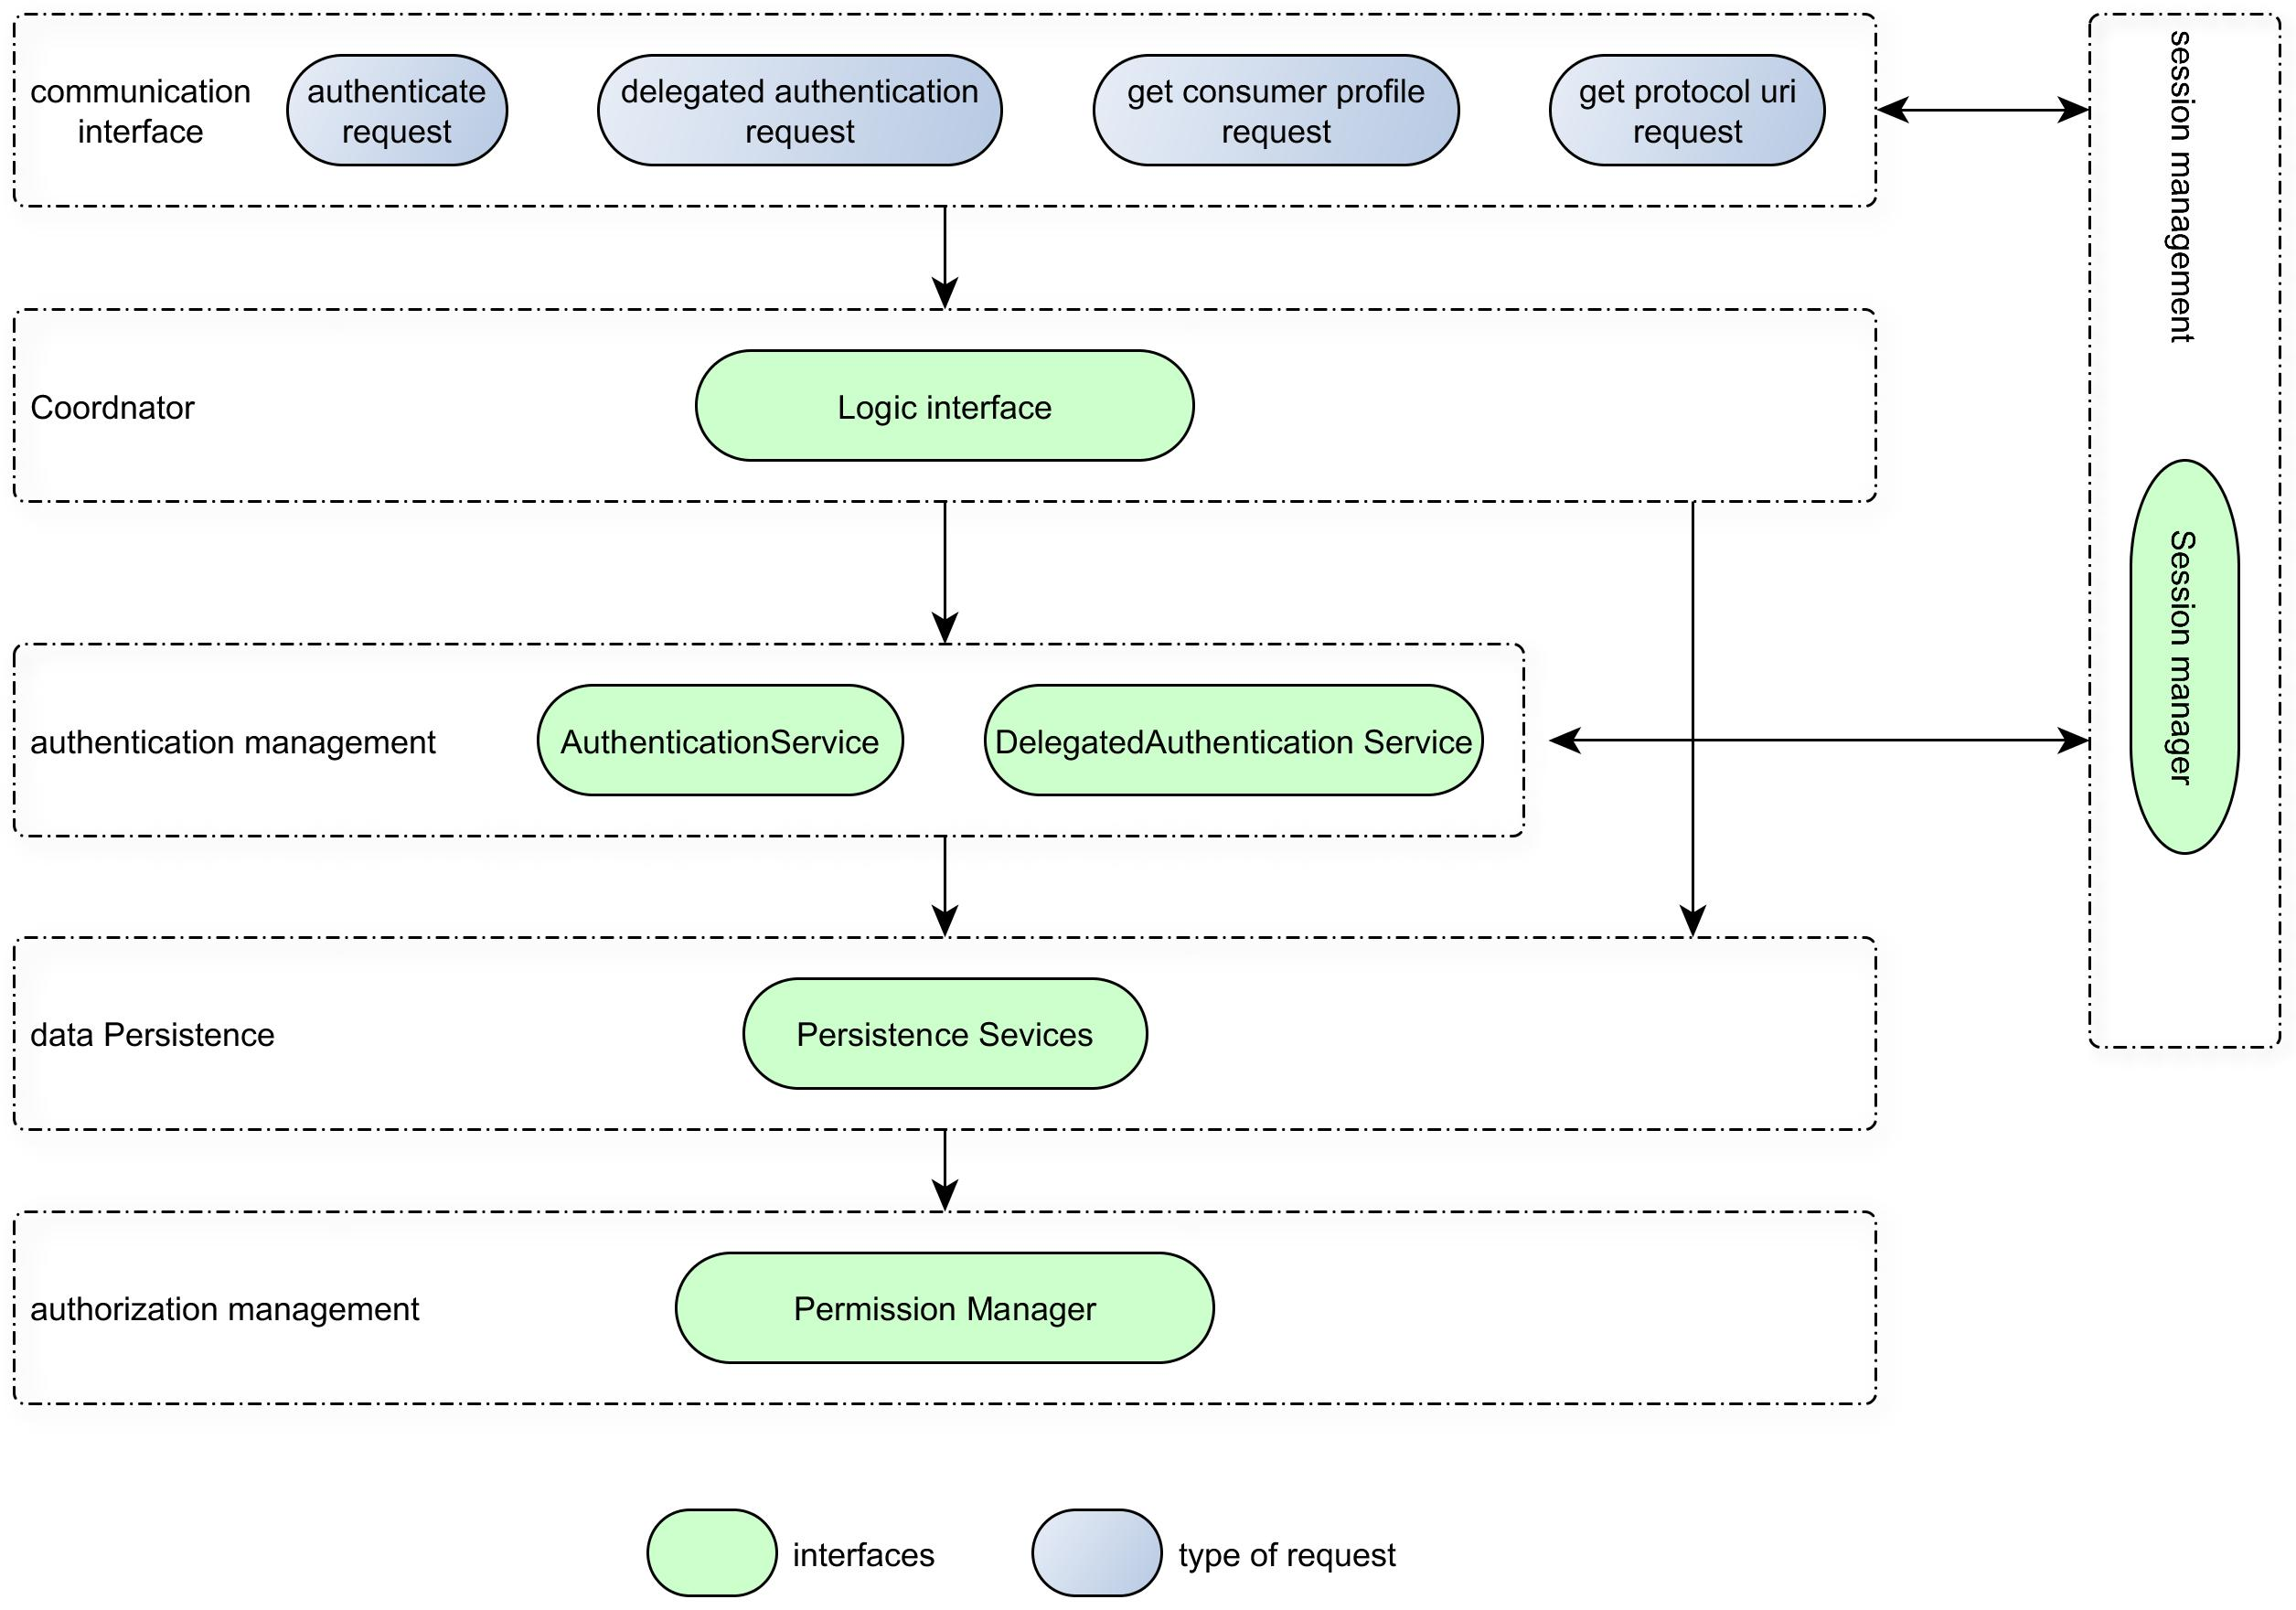
\includegraphics[angle=90,width=1\textwidth]{images/code_struct}
\end{figure}

\section{Session Management}
The session manager is the component whose role is to handle every session opened by users of the \emph{device cloud}. With "using", creating new session and removing existing ones is meant. 

A session must be understood as an authentication context, and contains among others the user opening the session, the time at which it is opened as well as a so-called sessionID. The users, when communicating with the server, just have to attach the sessionID. This approach has been preferred than the cookie based one, because combined with TLS/SSL, nobody can access the sessionID without the consent of the user. A cookie, in the other hand, has inherent weaknesses since it is a file stored on a hard drive.

Based on the time and sessionID information, the session manager includes also functions to retrieve an opened session from a sessionID and check the validity of a session (not outdated). This way, it allows the other components to check authentication information for any principal.

Most of the security leaks regarding sessions consists in the disclosure of the sessionID. Several weaknesses are known: session fixation (the sessionID of a user is set by the attacker. It can be done for example with server which accepts a new sessionID as HTTP parameter), session hijacking, XSS, session prediction (sessionID easy to guess) or weak sessionID storage.

The use of TLS/SSL and the non-use of cookies defeats any session hijacking attempts (sniffing cannot be done). Combined with a websocket communication and the fact that the session doesn't create new sessions based on request parameters, it also prevents session fixation. The java websocket architecture also erase any possibility of XSS attack (no scripting language is ever ran).
Session prediction is simply defeated by choosing a sufficient minimal length. In this case, the session ID contains at least 20 characters. Finally, weak session storage can compromise the session IDs if an attacker can access the storage. The implementation keeps the ids in the java virtual machine and never store them on the hard drive. Thus, this weakness is also handled.

\section{Persistence}

\subsection{DAO}
Each persistence service has been build with the same structure. This structure corresponds to a Data Access Object (DAO) design pattern. This pattern is now a widely accepted mechanism to abstract away the details of persistence in an application. Instead of having the domain logic communicate directly with the persistence system (database, file system, web service, etc), the domain logic speaks to a DAO layer instead. This DAO layer then communicates with the underlying persistence system or service.

The advantage of using such a DAO layer, is that if the underlying persistence system is changed, only the DAO layer should be adapted. The entity classes that are persisted (in this case the principals and the consumer profile), for example, can be kept. 

Thus, the persistence layer define a service per type of entity. The CRUD method can be then called from this service. A read operation on a consumer would then be achieved by the following call:

\lstset{language=Java}
\begin{lstlisting}
	PersistenceManager.getPersistenceService(EntityType.CONSUMER).get(consumerID)
\end{lstlisting}

It should be also remembered that entities can inherit from the AttachmentEntity interface, as shown in Tab. \ref{tab:entities_interface}. That means that file can be attached to an entity, and must be thus stored when the entity is persisted. 

Therefore, every persistence service adds a file-system storage mechanism to its standard storage mechanism (LDAP, database, etc).

\subsection{Principal Persistence}

As evoked earlier, persisting principals within a Domain can be done either with a dedicated database, or with an existing IAM solution.The Domain Operator will create new principals and verify the validity of incoming connections with this persistence system. For security purposes, the Domain Operator must be the only entity with access to this persistence system.

For this thesis, LDAP-based and dedicated database solutions have been analyzed. 

There aren't in fact many differences between the two approaches, since the most LDAP implementations are based on a backend database. However, one could sum up the plus and cons of both as depicted in \ref{tab:ldap_db}:

\begin{table}[h]
	\caption{A Comparison of LDAP and database solutions}
	\centering
	\label{tab:ldap_db}
	\begin{tabular}{|c|l|l|}
		\cline{2-3}
		\multicolumn{1}{c|}{} & 
		\multicolumn{1}{|c|}{\cellcolor{Gray}\textcolor{white}{\textbf{Database}}} & 
		\multicolumn{1}{|c|}{\cellcolor{Gray}\textcolor{white}{\textbf{LDAP}}} \\
		\hline
		\cellcolor{Gray}\textcolor{white}{\textbf{Plus}} &
		\pbox{0.4\linewidth}{
			\vspace{0.5em}
			\textbullet \quad support for transaction \\
			\textbullet \quad simpler
		} & 
		\pbox{0.4\linewidth}{
			\vspace{0.5em}
			\textbullet \quad very fast for read operations \\
			\textbullet \quad support for different authentication methods \\
			\textbullet \quad designed with security in mind
		} \\
		\hline
		\cellcolor{Gray}\textcolor{white}{\textbf{Cons}} &
		\pbox{0.4\linewidth}{
			\vspace{0.5em}
			\textbullet \quad offers a broader surface attack \\
		} & 
		\pbox{0.4\linewidth}{
			\vspace{0.5em}
			\textbullet \quad slow for write operations \\
			\textbullet \quad no transaction support \\
			\textbullet \quad heavier configuration
		} \\
		\hline
	\end{tabular}
\end{table}

The transaction support is a great deal in many system, as it is possible to rollback when an error occurs. But in the authentication framework, where only authentication must be performed, few operations are needed and none of them requires transaction. Indeed, those operations consist only in a get operation and a compare operation (for passwords), which is similar to a get operation. Besides, concurrent operation are unlikely to happen since the persistence system is designed to be used by only one user, the Domain Operator.

Another key decision factor here was the security considerations. The LDAP implementations are before all designed for authentication, and thus have a more robust architecture in the sense that they offer support for various security and authentication protocols and methods. In addition, a LDAP-based approach separates the data from the authentication, which allows for a better organization and offers a smaller attack surface.

Hence, a LDAP-based approach has been chosen.

\subsection{LDAP implementation}

A LDAP (Lightweight Directory Access Protocol) is originally a protocol to access and maintain directory information services. It has since evolved to become a norm, including a data model, a naming model, a functional model based on the protocol, a security model and a replication model.

the LDAP data model defines a hierarchical object tree structure, where every object has a RDN (relative distinguished name). The RDN is a set of key value pair, which is unique in the  object's branch (at the same level of the branch). The objects can then be uniquely identified within the whole tree by concatenating its RDN with its ancestors RDNs. This is the so-called distinguished name (DN). The objects composition (structure and attributes) are defined by schemes, which can be either standard, default or custom ones.

The LDAP tree, rendered in Fig \ref{ldap_tree} has been created with the use of 2 schemes, a standard and a custom one. The latter defines the following 4 classes: Operator, Vendor, Aggregator and Consumer as well as their attributes. The structure of the tree follows then simply the underlying logic: all above-listed principals belong to their organizational unit (customers, etc) defined by the standard scheme, and constitute in turn the User Directory.

To enhance re-usability, the tree has also as root element an organization (like TU Berlin) and a domain name, in this case userdirectory.devicecloud. Those two objects are also defined by the standard scheme. In the end, a Consumer will then be identified by the following Distinguished Name:

\quad \quad \textit{entityID=consumerID, ou=consumers, o=TU Berlin, dc=userdirectory, dc=devicecloud}

The LDAP server used is an OpenLDAP Server, mainly because it offers a good documentation and worldwide commercial support. It is also highly configurable. The configuration might be made easier with other LDAP server, like ApacheDS or OpenDJ, but is also shipped with client applications (respectively Apache Directory Studio and OpenAM), which allows to easily manage users and groups, defined in standard schemes. Since the users of the \emph{device cloud} are defined with a custom scheme, those features are not required.

Finally, the security measures defined in \ref{LDAP_security} have also been implemented. One can connect to the LDAP Server without use TLS/SSL, but any action requires to be authenticated, and the only way to authenticate has been configured as Certificate authentication.

The configuration of the LDAP might be tedious, because it involves many different steps (creation of LDAP, configuring basic properties like communication port or logging, adding custom schemes, configuring ssl, setting the right to the legitimate entities, restraining right of all others, etc) and because the error messages of the LDAP are rarely descriptive enough. Consequently, a docker file has been created, that allows for a quick deployment of a working LDAP server. 

Basic properties like communication port or IP of the User Directory machine must be first set in the docker file, a simple docker run deploys then the LDAP server.


\begin{figure}[tbhp]
	\centering
	\caption{Structure of the LDAP tree}
	\label{ldap_tree}
	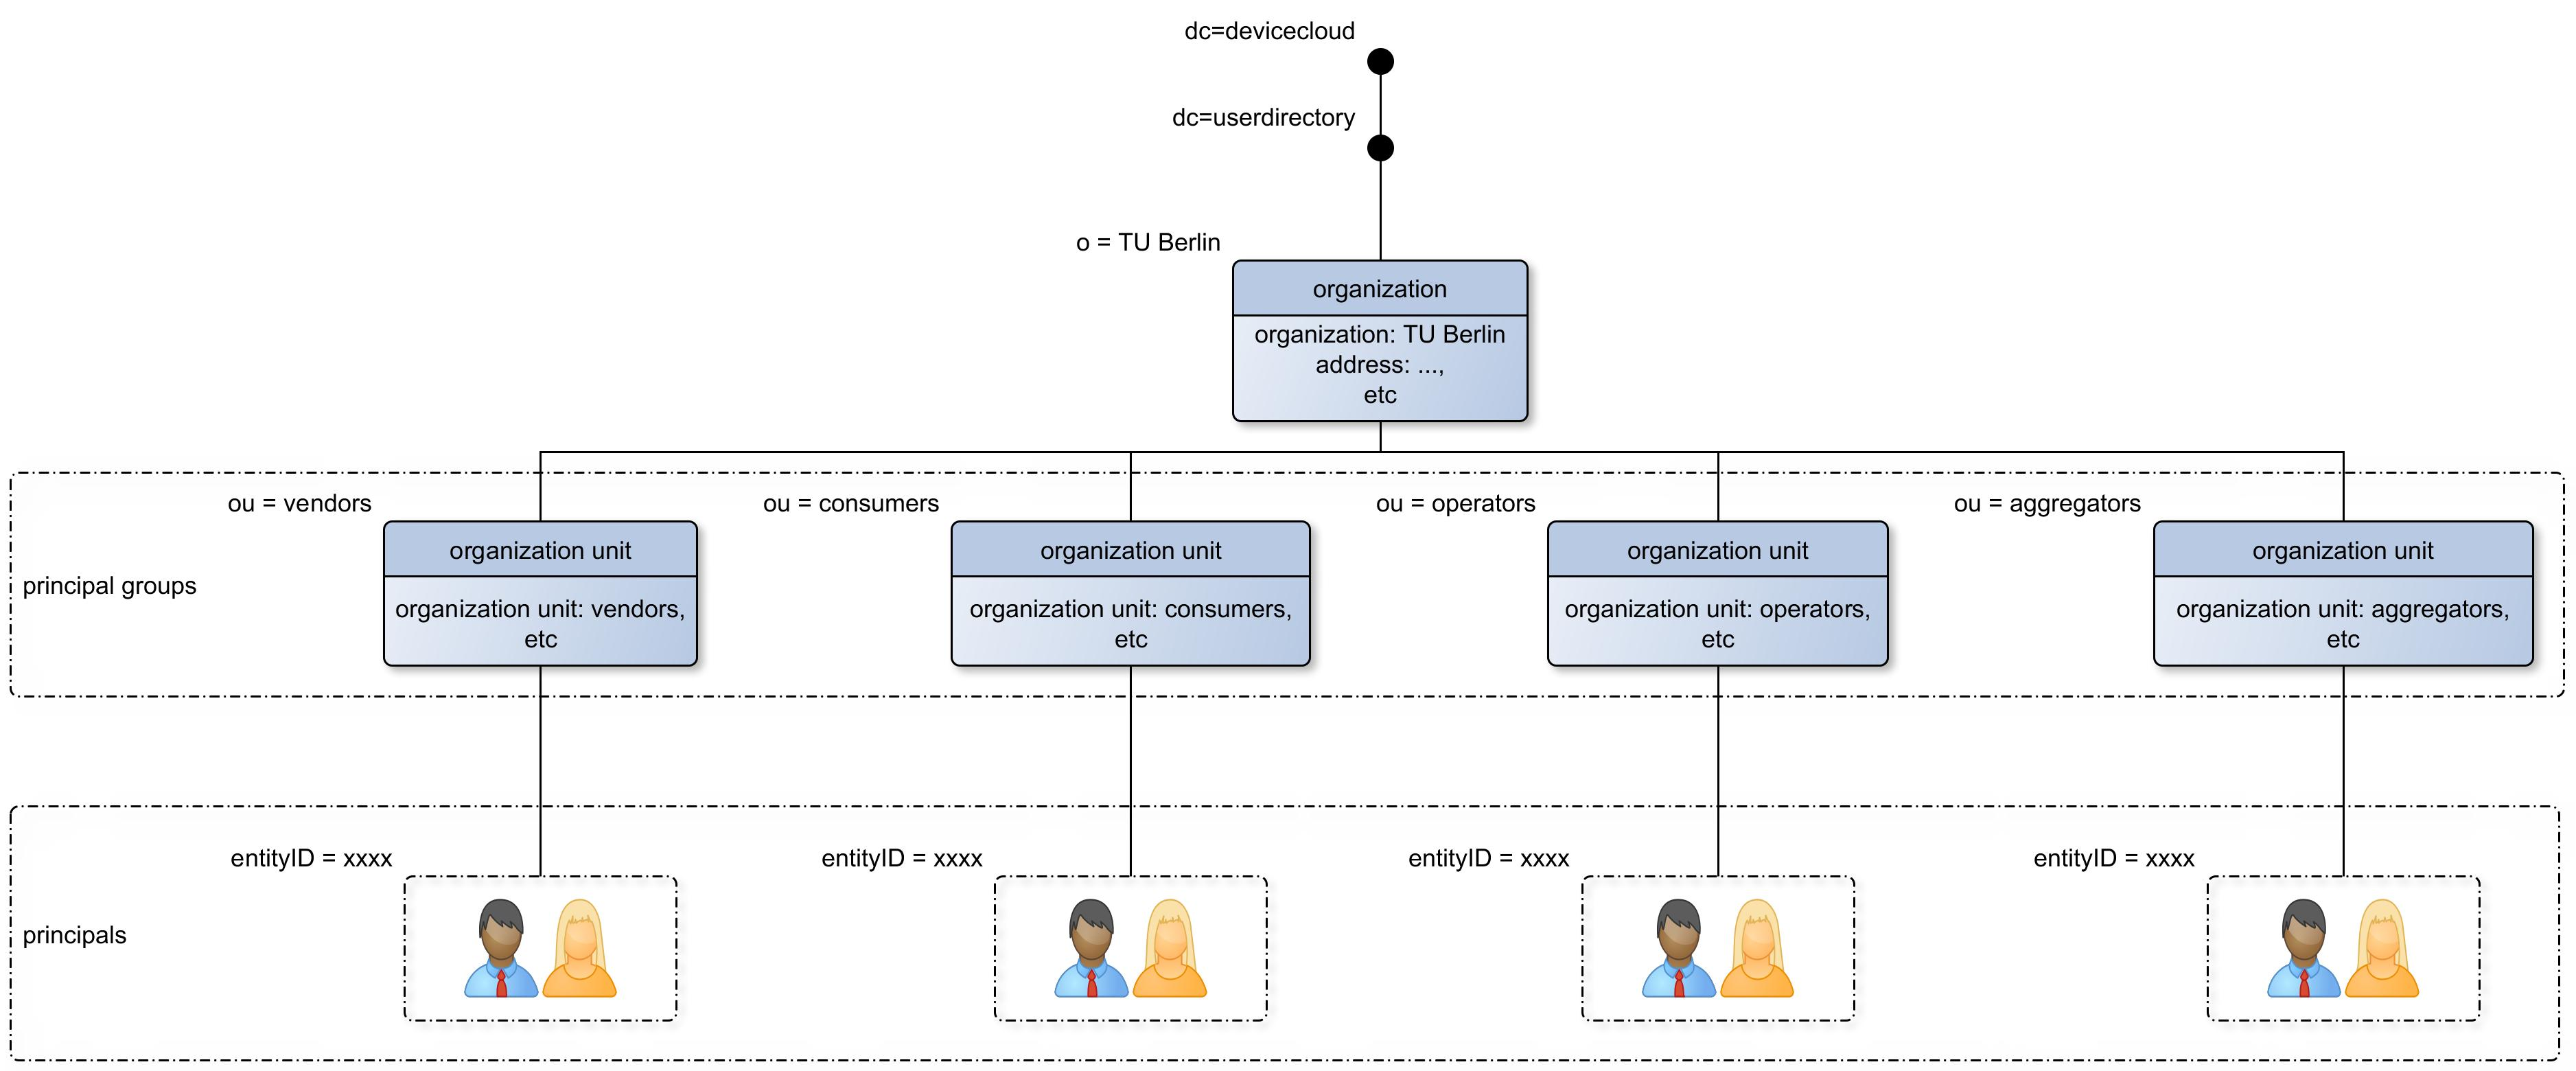
\includegraphics[angle=90,height=\textheight]{images/ldap_tree}
\end{figure}

\subsection{Entities and their authorization properties persistence}

A dedicated database has also been used for the Consumer Profile. This database was part of the previous work done on the \emph{device cloud}, as entities had already been defined (see section \ref{sec:02_entities}). 

However, this database has not yet been secured as required in section \ref{sec:03_database}. Instead, a in-memory database has been used, for testing purposes. It should be therefore be ensured that those requirements are met when deploying.

\section{Testing}
This sections explains now how the User Directory has been tested. By User Directory, the result of the four methods specified in \ref{sec:04_framework} is meant.

Testing the framework can be tedious, because it can't just be be done with unit tests for example, since an end-to-end connection must be established (an End-User authenticates to its IdP for example, over a SSL secured channel). Every test must therefore have its own configuration, with certificates, private keys, etc.

For a better understanding of the problem, the workflow of the direct and delegated authentication testing logic, on which the conducted tests are based, is rendered in Fig. \ref{fig:tests_1}: there are for example two possibilities for the authentication to fail: either a bad certificate or bad request parameters. A certificate can for example be not valid because the it is not signed by the correct CA, or because the information contained is false (it contains among other the ID of the entity using it). 

This leads to the creation of $ 3 \times 4 = 12 $ certificates and public/private key pairs only for the principals (1 valid and 2 false for 4 types of principals: Consumer, Aggregator, Vendor and Operator). When considering also IdPs and clients, the configuration becomes really complex.

However, every test have been successfully performed. It can be thus concluded that the SSL environment has been correctly configured and that the authentications methods behave as expected. 

Once the authentication methods tested, the configuration for the Get Protocol URI and Get Consumer Profile was already set up. Therefore, the specifications given in Tab. \ref{tab:access_control} were verified more easily.

\begin{figure}[!tbh]
	\centering
	\subfloat[direct authentication testing structure][direct authentication testing structure]{
		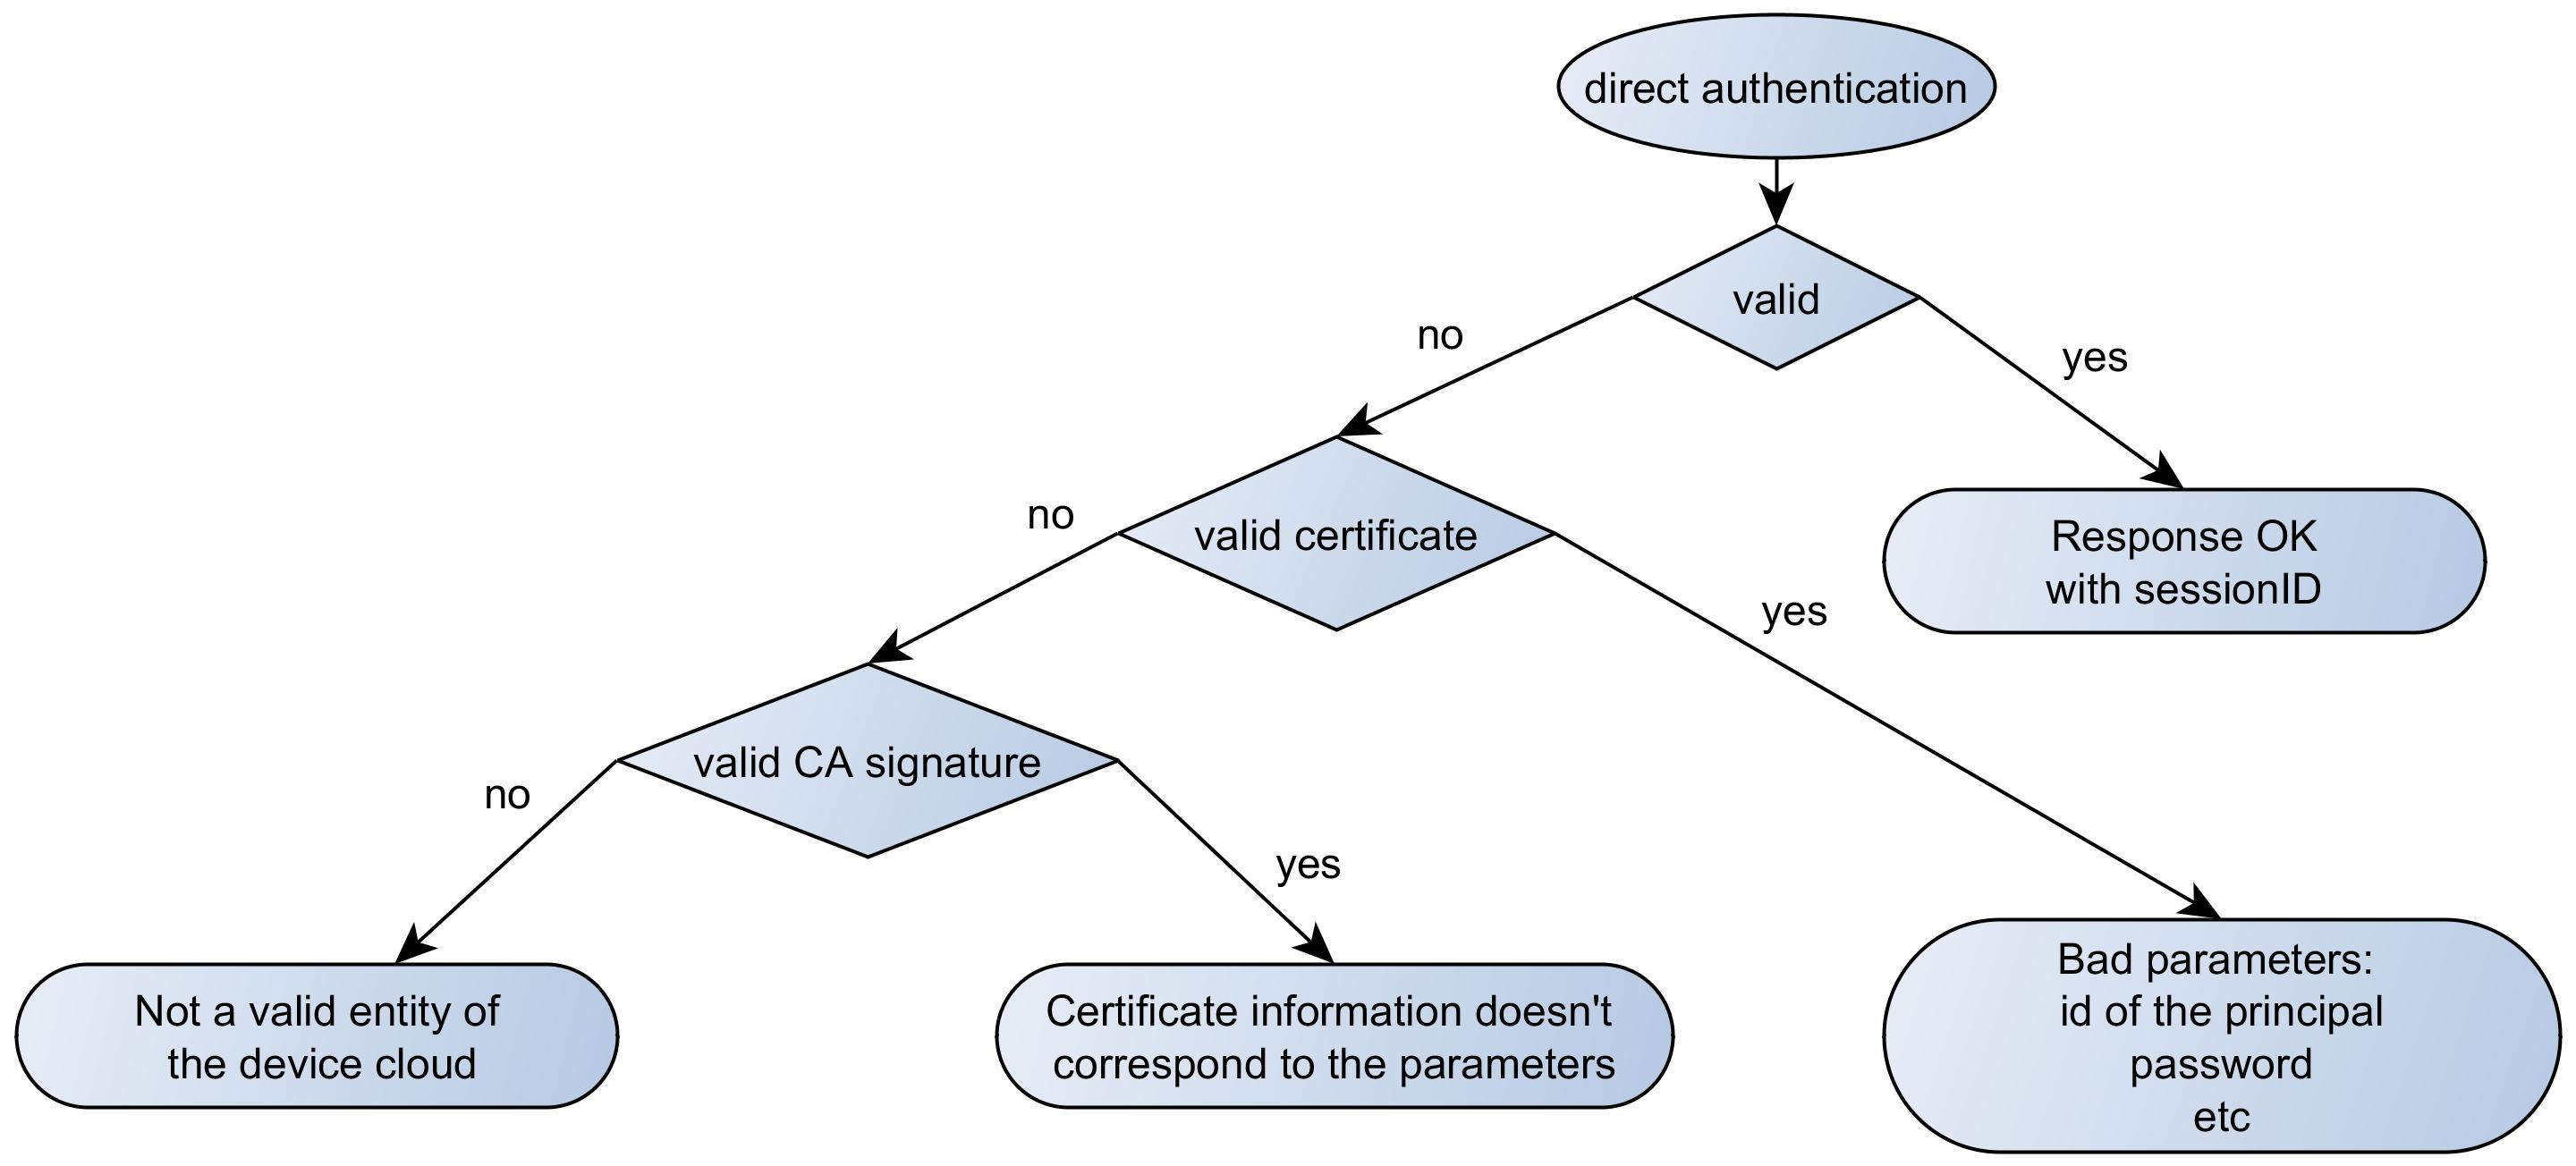
\includegraphics[width=\textwidth]{images/tests}
		\label{fig:tests_1}}
	\qquad
	\subfloat[delegated authentication testing structure][delegated authentication testing structure]{
		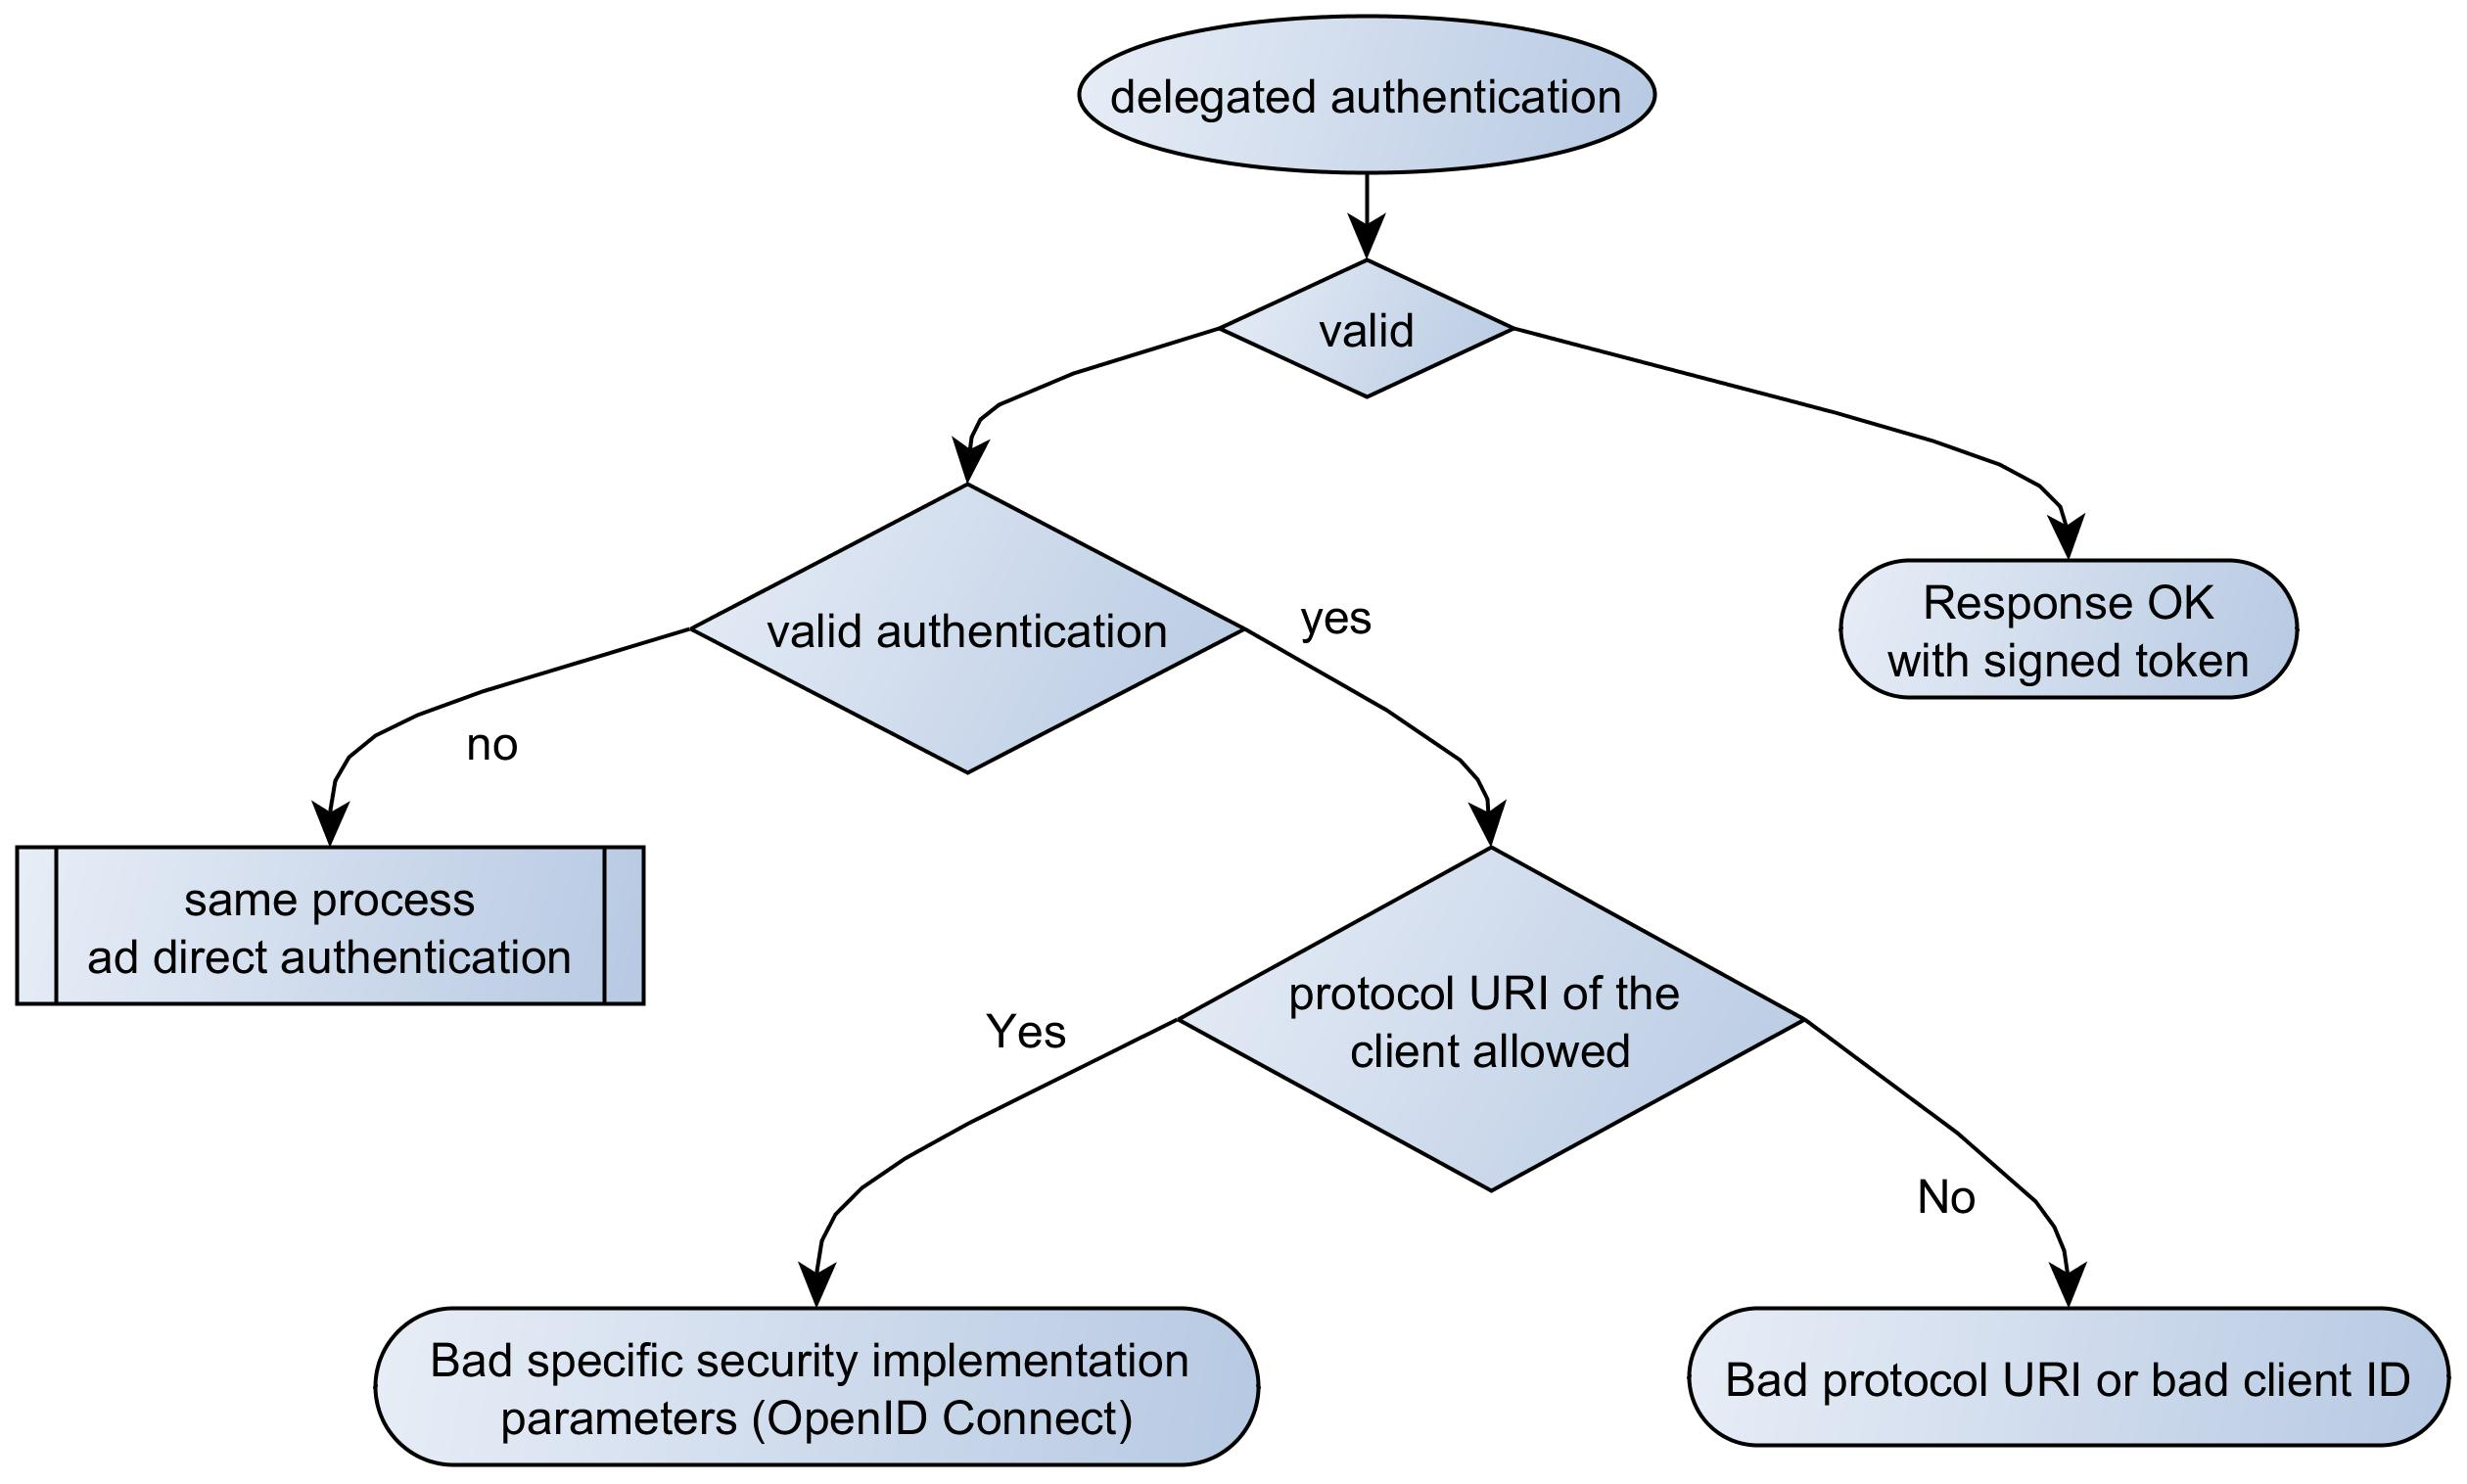
\includegraphics[width=\textwidth]{images/tests_2}
		\label{fig:tests_2}}
	\caption{Tests structure}
	\label{fig:tests}
\end{figure}



